\begin{flushleft}
    \fontsize{16}{20}\selectfont
    \section*{CHƯƠNG 3: NHẬN XÉT, ĐÁNH GIÁ THỰC TRẠNG}
    \addcontentsline{toc}{section}{CHƯƠNG 3: NHẬN XÉT, ĐÁNH GIÁ THỰC TRẠNG}
    \fontsize{13}{20}\selectfont
    \setcounter{section}{3}
    \setcounter{subsection}{0}
    \subsection{Giới thiệu về YOLO}
    \fontsize{13}{20}\selectfont\paragraph{}
    YOLO (You Only Look Once) là một trong những thuật toán hàng đầu trong việc nhận diện vật thể. Thuật toán này nổi bật nhờ vào khả năng thực hiện nhận diện rất nhanh chóng và hiệu quả, ngay cả trên những tập dữ liệu lớn và phức tạp. Ý tưởng chính của YOLO là biến bài toán nhận diện vật thể thành một bài toán hồi quy duy nhất, thay vì tiếp cận từng bước như các phương pháp truyền thống.\\
    \begin{figure}[h]
        \centering
        
\includegraphics[width=0.2\textwidth]{images/YOLO.jpg}
        \caption{Logo YOLOv5}\label{fig:logo_YOLO}
    \end{figure}
    \textbf{Nguyên Lý Hoạt Động của YOLO:}\\
    \begin{itemize}
            \item Phân Chia Ảnh: \\Ảnh đầu vào được chia thành một lưới SxS
            \item Dự Đoán Bounding Boxes và Xác Suất:\\Mỗi ô trong lưới dự đoán số lượng các bounding boxes (khung chứa) và xác suất để mỗi khung chứa một vật thể.
            \item Kết Hợp Bounding Boxes: \\Các bounding boxes có xác suất cao sẽ được kết hợp và lọc để đưa ra dự đoán cuối cùng.
    \end{itemize}
    Các phiên bản khác nhau của YOLO (như YOLOv1, YOLOv2, YOLOv3, YOLOv4) đã mang đến nhiều cải tiến về mặt kiến trúc và hiệu năng, nhưng tất cả đều dựa trên nguyên lý cơ bản này.\\
    \textbf{YOLOv5}\\
    YOLOv5 là phiên bản mới của dòng thuật toán YOLO và được phát triển bởi công ty Ultralytics. YOLOv5 kế thừa các ưu điểm của các phiên bản trước và đưa ra nhiều cải tiến quan trọng, cả về mặt tốc độ lẫn độ chính xác.\\
    \textbf{YOLOv5}\\
    \fontsize{13}{20}\selectfont\subsubsection{Các Đặc Điểm Nổi Bật của YOLOv5:}
    \begin{itemize}
        \item Kiến Trúc Nhẹ và Hiệu Quả: YOLOv5 được thiết kế nhẹ nhàng và hiệu quả, cho phép triển khai dễ dàng trên các thiết bị có phần cứng hạn chế.
        \item Cải Tiến về Huấn Luyện: YOLOv5 sử dụng các kỹ thuật mới như Mosaic Augmentation, auto-learning bounding box anchors, và tích hợp sẵn các chiến lược training tốt nhất như cosine learning rate annealing.
        \item Tối Ưu Hóa Hiệu Năng: YOLOv5 có các phiên bản nhỏ gọn (YOLOv5s), trung bình (YOLOv5m), lớn (YOLOv5l), và rất lớn (YOLOv5x) để phù hợp với nhiều loại ứng dụng khác nhau.
        \item Khả Năng Chuyển Giao (Transfer Learning): YOLOv5 hỗ trợ tốt cho việc fine-tuning mô hình trên các tập dữ liệu riêng biệt, giúp dễ dàng tùy chỉnh cho các bài toán cụ thể.
    \end{itemize}
    \fontsize{13}{20}\selectfont\subsubsection{Quá Trình Hoạt Động của YOLOv5}
    \begin{itemize}
        \item Tiền Xử Lý: Ảnh đầu vào được điều chỉnh kích thước và áp dụng các kỹ thuật tăng cường dữ liệu (data augmentation).
        \item Trích Xuất Đặc Trưng: Sử dụng một backbone CNN (như CSPDarknet) để trích xuất các đặc trưng từ ảnh.
        \item Đầu Ra của Mạng: Mạng chia ảnh thành các lưới và dự đoán bounding boxes cùng với xác suất cho từng lưới.
        \item Hậu Xử Lý: Sử dụng các kỹ thuật như Non-Maximum Suppression (NMS) để lọc và kết hợp các bounding boxes, đưa ra dự đoán cuối cùng.
    \end{itemize}
    \fontsize{13}{20}\selectfont\subsubsection{Cải tiến và hiệu năng}
    \begin{itemize}
        \item Tốc Độ và Độ Chính Xác: YOLOv5 vượt trội ở khả năng xử lý ảnh thời gian thực với độ chính xác cao.
        \item Thân Thiện với Người Dùng: Được triển khai bằng PyTorch, YOLOv5 dễ dàng tùy chỉnh và tích hợp vào các hệ thống khác.
        \item Khả Năng Mở Rộng: YOLOv5 có thể mở rộng và tinh chỉnh cho nhiều loại ứng dụng từ giám sát an ninh đến phân tích y tế.
    \end{itemize}
    \subsubsection{Ứng Dụng của YOLOv5}
    \begin{itemize}
        \item Giám Sát An Ninh: Nhận diện các hành vi bất thường hoặc phát hiện kẻ xâm nhập.
        \item Y Tế: Phân tích hình ảnh y tế để phát hiện bệnh tật.
        \item Giao Thông: Phân tích lưu lượng giao thông, nhận diện phương tiện.
        \item Thương Mại Điện Tử: Tự động gán nhãn sản phẩm và quản lý kho hàng.
    \end{itemize}
    YOLOv5 không chỉ tiếp tục di sản của dòng YOLO mà còn mở rộng khả năng của nó, đem lại những tiến bộ vượt bậc trong lĩnh vực nhận diện vật thể. Với sự phát triển liên tục, YOLOv5 hứa hẹn sẽ tiếp tục là công cụ mạnh mẽ và hữu ích cho các ứng dụng trong tương lai.
    \subsection{Giới thiệu về OpenCV}
    OpenCV (Open Source Computer Vision Library) là một thư viện mã nguồn mở mạnh mẽ, được thiết kế để cung cấp các công cụ và giải thuật cho xử lý ảnh và thị giác máy tính. Được phát triển bởi Intel vào năm 1999, OpenCV nhanh chóng trở thành một trong những thư viện phổ biến nhất trong lĩnh vực xử lý ảnh và thị giác máy tính, nhờ tính linh hoạt, hiệu suất cao và khả năng hỗ trợ đa nền tảng.\\
    \begin{figure}[h]
        \centering
        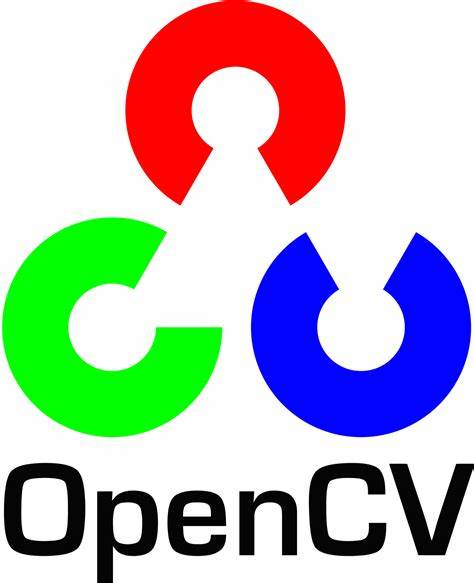
\includegraphics[width=0.2\textwidth]{images/OIP.jpg}
        \caption{Logo OpenCV}\label{fig:logo_cv2}
    \end{figure}
    \subsubsection{Các Đặc Điểm Nổi Bật của OpenCV}
    \begin{itemize}
        \item Đa Nền Tảng: Hỗ trợ Windows, Linux, macOS, Android và iOS.
        \item Hỗ Trợ Ngôn Ngữ Đa Dạng: Python, C++, Java và nhiều ngôn ngữ lập trình khác.
        \item Thư Viện Đa Dạng: Cung cấp hơn 2500 thuật toán và hàm xử lý ảnh, bao gồm nhận diện khuôn mặt, phát hiện chuyển động, phân đoạn ảnh, và nhiều hơn nữa.
        \item Hiệu Suất Cao: Được tối ưu hóa cao để sử dụng các phần cứng như CPU và GPU.
    \end{itemize}
    \subsubsection{Vẽ với OpenCV}
    OpenCV cung cấp nhiều hàm vẽ cơ bản để tạo và xử lý các hình ảnh. Các hàm vẽ này bao gồm vẽ đường thẳng, hình chữ nhật, hình tròn, đa giác và thêm văn bản lên ảnh.\\
    \begin{itemize}
        \item cv2.line(): Vẽ đường thẳng.
        \item cv2.rectangle(): Vẽ hình chữ nhật.
        \item cv2.circle(): Vẽ hình tròn.
        \item cv2.ellipse(): Vẽ hình ellipse.
        \item cv2.polylines(): Vẽ đa giác.
        \item cv2.putText(): Thêm văn bản lên ảnh.
    \end{itemize}
    \subsubsection{Các Bước Thao Tác với Camera}
    \begin{itemize}
        \item Mở Camera: Sử dụng cv2.VideoCapture() để mở camera.
        \item Đọc Khung Hình: Sử dụng cap.read() để đọc từng khung hình từ camera.
        \item Thị Khung Hình: Sử dụng cv2.imshow() để hiển thị khung hình.
        \item Lý Khung Hình: Áp dụng các thuật toán xử lý ảnh lên từng khung hình.
        \item Video: Sử dụng cv2.VideoWriter() để lưu lại video nếu cần.
    \end{itemize}
    \subsubsection{Ứng Dụng của OpenCV}
    OpenCV được sử dụng rộng rãi trong nhiều lĩnh vực khác nhau: \\
    Giám Sát An Ninh: Phát hiện chuyển động, nhận diện khuôn mặt.
    Y Tế: Phân tích hình ảnh y tế, nhận diện bệnh lý.
    Giao Thông: Phân tích lưu lượng giao thông, nhận diện biển số xe.
    Thương Mại Điện Tử: Quản lý kho hàng, phân loại sản phẩm.


\end{flushleft}
